\documentclass[journal,12pt,onecolumn]{IEEEtran}
\usepackage[top=0.2in,bottom=1in,left=1in,right=1in]{geometry}
\usepackage{cite}
\usepackage{graphicx}
\usepackage{amsmath,amssymb,amsfonts,amsthm}
\usepackage{algorithmic}
\usepackage{graphicx}
\usepackage{textcomp}
\usepackage{xcolor}
\usepackage{txfonts}
\usepackage{listings}
\usepackage{enumitem}
\usepackage{mathtools}
\usepackage{gensymb}
\usepackage{comment}
\usepackage[breaklinks=true]{hyperref}
\usepackage{tkz-euclide} 
\usepackage{listings}
\usepackage{gvv}                                        
%\def\inputGnumericTable{}                                 
\usepackage[latin1]{inputenc} 
\usetikzlibrary{arrows.meta, positioning}
\usepackage{xparse}
\usepackage{color}                                            
\usepackage{array}                                            
\usepackage{longtable}                                       
\usepackage{calc}                                             
\usepackage{multirow}
\usepackage{multicol}
\usepackage{caption}
\usepackage{hhline}                                           
\usepackage{ifthen}                                           
\usepackage{lscape}
\usepackage{tabularx}
\usepackage{array}
\usepackage{float}
\newtheorem{theorem}{Theorem}[section]
\newtheorem{problem}{Problem}
\newtheorem{proposition}{Proposition}[section]
\newtheorem{lemma}{Lemma}[section]
\newtheorem{corollary}[theorem]{Corollary}
\newtheorem{example}{Example}[section]
\newtheorem{definition}[problem]{Definition}
\newcommand{\BEQA}{\begin{eqnarray}}
\newcommand{\EEQA}{\end{eqnarray}}
\usepackage{float}
%\newcommand{\define}{\stackrel{\triangle}{=}}
\theoremstyle{remark}
\usepackage{circuitikz}
\usepackage{tikz}
\usepackage{wrapfig}
\graphicspath{{figs/}}                                                                       
\title{Graduate Aptitude Test in Engineering 2017}

\author{EE25BTECH11023-Venkata Sai}
\begin{document}
\noindent
\maketitle
\textit{Duration:} Three Hours \hfill \textit{Maximum Marks:} 100

\begin{enumerate}

\item Divergence of the curl of a twice differentiable continuous vector function is:
\begin{enumerate}
\begin{multicols}4
\item unity
\item infinity
\item zero
\item a unit vector
\end{multicols}
\end{enumerate}
\hfill (GATE PI 2017)

\item For two non-zero vectors $\bar{A}$ and $\bar{B}$, if $\bar{A} + \bar{B}$ is perpendicular to $\bar{A} - \bar{B}$, then:
\begin{enumerate}
\item the magnitude of $\bar{A}$ is twice the magnitude of $\bar{B}$
\item the magnitude of $\bar{A}$ is half the magnitude of $\bar{B}$
\item $\bar{A}$ and $\bar{B}$ cannot be orthogonal
\item the magnitudes of $\bar{A}$ and $\bar{B}$ are equal
\end{enumerate}
\hfill (GATE PI 2017)

\item For an orthogonal matrix $Q$, the valid equality is:
\begin{enumerate}
\begin{multicols}{4}
\item $Q^{T} = Q^{-1}$
\item $Q = Q^{-1}$
\item $Q = Q$
\item $\det(Q) = 0$
\end{multicols}
\end{enumerate}
\hfill (GATE PI 2017)

\item The product of a complex number $z = x + i y$ and its complex conjugate $\bar{z}$ is:
\begin{enumerate}
\begin{multicols}{4}
\item $x^{2}$
\item $y^{2}$
\item $x^{2} - y^{2}$
\item $x^{2} + y^{2}$
\end{multicols}
\end{enumerate}
\hfill (GATE PI 2017)

\item Using Simpson's $\frac{1}{3}$ rule for numerical integration, the consecutive points are joined by a
\begin{enumerate}
\begin{multicols}{2}
\item line
\item parabola
\item polynomial with power 3
\item polynomial with power $\frac{1}{3}$
\end{multicols}
\end{enumerate}
\hfill (GATE PI 2017)

\item For a two-dimensional state of stress defined as $\sigma_{xx} = \sigma_{yy} = \tau_{xy} = S$, the Mohr's circle of stress has:
\begin{enumerate}
\item center at $\brak{S, 0}$ and radius $S$
\item center at $\brak{0, 0}$ and radius $S$
\item center at $\brak{S, 0}$ and radius $0$
\item center at $\brak{\frac{S}{2}, 0}$ and radius $2S$
\end{enumerate}
\hfill (GATE PI 2017)

\item A specimen of steel has yield strength of 700 MPa. It is subjected to a state of plane stress with $\sigma_1 = 500$ MPa and $\sigma_2 = 0$. The factor of safety according to the von-Mises theory of failure is \dots

\hfill (GATE PI 2017) 


\item The inside and outside radii of a thick-walled cylindrical pressure vessel are denoted by $a$ and $b$, respectively. If the vessel is subjected to an internal pressure $P$, then the magnitude of the radial stress $\sigma_r$ is:
\begin{enumerate}
\item zero at $r = a$ and maximum at $r = b$
\item maximum at $r = a$ and zero at $r = b$
\item constant over the entire thickness
\item zero at both $r = a$ and $r = b$
\end{enumerate}
\hfill (GATE PI 2017)

\item A metallic cylindrical casing of an exhaust pipe has inner radius $50$ mm and wall thickness $7$ mm. If the thermal conductivity of the material is 50 W/m-K, then the thermal resistance of the casing (in K/kW) is \dots (up to three decimal places).  

\hfill (GATE PI 2017)

\item In Value Engineering approach, the value of the product is:
\begin{enumerate}
\item inversely proportional to its functions and directly proportional to its cost
\item directly proportional to its functions and inversely proportional to its cost
\item inversely proportional to its functions as well as its cost
\item directly proportional to its functions as well as its cost
\end{enumerate}
\hfill (GATE PI 2017)

\item Match the ASME process chart symbols with their correct description: \\

\begin{enumerate}

    \item[] (P) $\bigcirc$  \quad 1.STORAGE\\
    \item[] (Q) $\longrightarrow$ \quad 2.TRANSPORTATION\\
    \item[] (R) $\square$ \quad 3. OPERATION \\
    \item[] (S) $\nabla$ \quad 4.DELAY \\
    \item[] (T) \textbf{D}  \quad 5.INSPECTION \\
\end{enumerate}


\begin{enumerate}
\begin{multicols}{2}
\item P-3, Q-4, R-1, S-5, T-2
\item P-4, Q-2, R-5, S-1, T-3
\item P-3, Q-2, R-5, S-1, T-4
\item P-1, Q-5, R-3, S-2, T-4
\end{multicols}
\end{enumerate}
\hfill (GATE PI 2017)

\item In Glass Fiber Reinforced Plastic (GFRP) composites with long fibers, the role of matrix is to:  

(P) support and transfer the stresses to the fibers  

(Q) reduce propagation of cracks  

(R) carry the entire load  

(S) protect the fibers against damage  

The correct statements are:
\begin{enumerate}
\begin{multicols}{4}
\item P, Q and R
\item Q, R and S
\item P, Q and S
\item P, R and S
\end{multicols}
\end{enumerate}
\hfill (GATE PI 2017)

\item Turning, drilling, boring and milling are common machining operations. Among these, the operation(s) performed by a single point cutting tool is(are):
\begin{enumerate}
\begin{multicols}{2}
\item turning only
\item drilling and milling only
\item turning and boring only
\item boring only
\end{multicols}
\end{enumerate}
\hfill (GATE PI 2017)

\newpage
\item In chemical machining, the etch factor is expressed as:
\begin{enumerate}
\begin{multicols}{2}
\setlength{\itemsep}{0.3cm}
\item $\frac{\text{undercut}}{\text{depth of cut}}$
\item $\frac{\text{depth of cut}}{\text{undercut}}$ 
\item $\frac{\text{workpiece wear}}{\text{tool wear}}$
\item $\frac{\text{tool wear}}{\text{workpiece wear}}$
\end{multicols}
\end{enumerate}
\hfill (GATE PI 2017)
\newline
\item A Shewhart $\bar{X}$-chart was developed for an in-control process. Considering the probability of a point falling outside the $3\sigma$ control limits as $0.0026$, the value of average run length for this chart is:  
\dots   

\hfill (GATE PI 2017)

\item Accuracy of a measuring instrument is expressed as:
\begin{enumerate}
\item $\text{true value} - \text{measured value}$
\item $\text{measured value} - \text{true value}$
\item $1 - \frac{\text{true value} - \text{measured value}}{\text{true value}}$
\item $1 + \frac{\text{true value} - \text{measured value}}{\text{true value}}$
\end{enumerate}
\hfill (GATE PI 2017)

\item The operating characteristic curves of three single sampling plans X, Y and Z with same lot size and acceptance number are shown in the figure.

\begin{figure}[H]
    \centering
    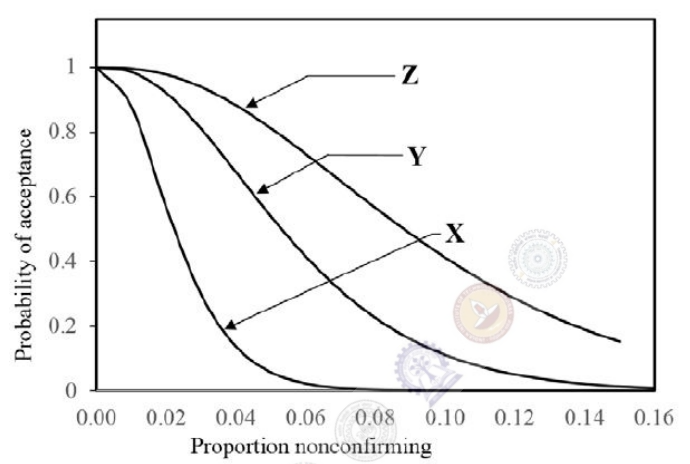
\includegraphics[width=0.5\columnwidth]{figs/fig1.png}
    \caption{}
    \label{fig:placeholder}
\end{figure} 


Based on these curves, the correct relationship of the plans with respect to sample size is:
\begin{enumerate}
\item sample size of X $<$ sample size of Y $<$ sample size of Z
\item sample size of X $=$ sample size of Y $=$ sample size of Z
\item sample size of X $>$ sample size of Y $>$ sample size of Z
\item sample size of X $>$ sample size of Y $<$ sample size of Z
\end{enumerate}
\hfill (GATE PI 2017)

\item In carbon dioxide molding process, the binder used is:
\begin{enumerate}
\item Sodium bentonite
\item Calcium bentonite
\item Sodium silicate
\item Phenol formaldehyde
\end{enumerate}

\hfill (GATE PI 2017)

\item A steel wire of $2$ mm diameter is to be drawn from a wire of $5$ mm diameter.  
The value of true strain developed is:  
\dots (up to three decimal places)  

\hfill (GATE PI 2017)

\item In gas tungsten arc welding process, the material coated on pure tungsten electrode  
to enhance its current carrying capacity is:
\begin{enumerate}
\begin{multicols}{4}
\item Titanium
\item Manganese
\item Radium
\item Thorium
\end{multicols}
\end{enumerate}

\hfill (GATE PI 2017)

\item In powder metallurgy, the process \textit{atomization} refers to a method of:
\begin{enumerate}
\item producing powders
\item compaction of powders
\item sintering of powder compacts
\item blending of metal powders
\end{enumerate}

\hfill (GATE PI 2017)

\item The ideal stress\--strain behavior for a completely brittle material during tensile testing up to failure is described by:
\begin{figure}[H]
    \centering
    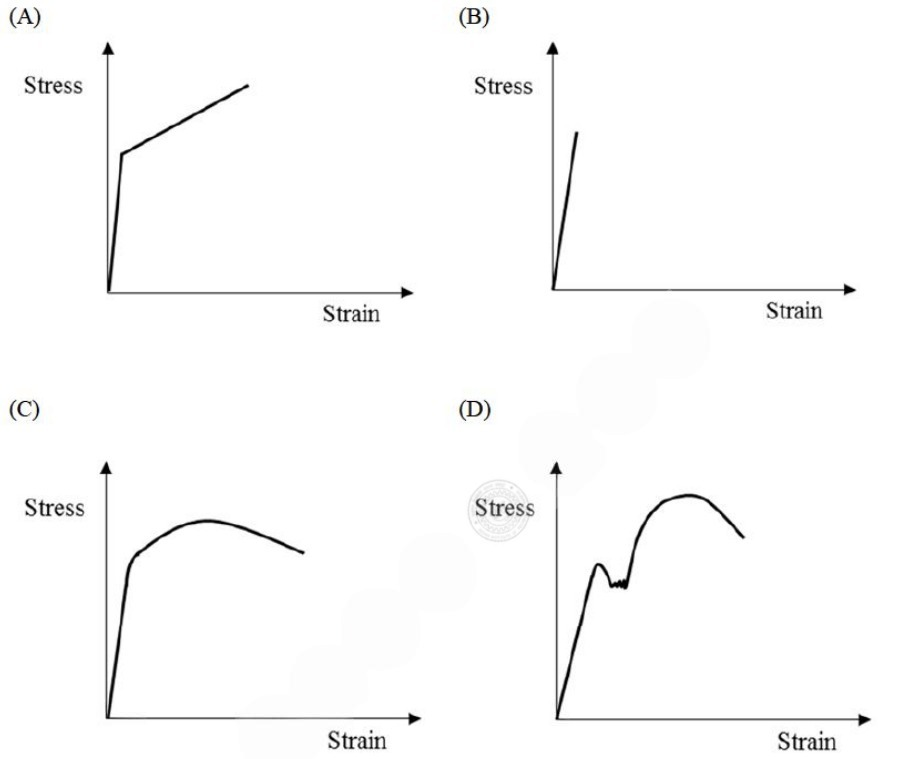
\includegraphics[width=1\columnwidth]{fig2.png}
    \caption{}
    \label{fig:placeholder}
\end{figure}

\hfill (GATE PI 2017)

\item With reference to the Iron\--Carbon equilibrium phase diagram, the crystal structure of $0.3\%$ plain carbon steel at $1100^\circ$C is:
\begin{enumerate}
\begin{multicols}{4}
\item HCP
\item BCT
\item BCC
\item FCC
\end{multicols}
\end{enumerate}

\hfill (GATE PI 2017)

\item If $E$ is the modulus of elasticity in GPa, $G$ is the shear modulus in GPa and $\nu$ is the Poisson's ratio of a linear elastic isotropic material, the three parameters are related as:
\begin{enumerate}
\begin{multicols}{2}
\item $E = G(1 - 2\,\nu)$
\item $E = 2G(1 - \nu)$
\item $E = G(1 + 2\,\nu)$
\item $E = 2G(1 + \nu)$
\end{multicols}
\end{enumerate}

\hfill (GATE PI 2017)

\item A machined surface with standard symbols indicating the surface texture is shown in the figure (all dimensions in $\mu$m).  

\begin{figure}[H]
    \centering
    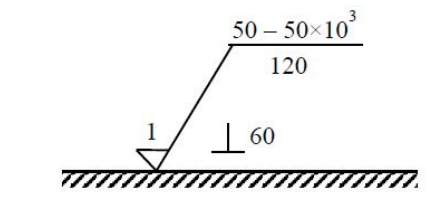
\includegraphics[width=0.5\columnwidth]{fig3.png}
    \caption{}
    \label{fig:placeholder}
\end{figure}

The waviness height (in $\mu$m) of the surface is:
\begin{enumerate}
\begin{multicols}{4}
\item 1
\item 50
\item 60
\item 120
\end{multicols}
\end{enumerate}

\hfill (GATE PI 2017)

\item The improper integral $\int_{0}^{\infty} e^{-2t} \, dt$ converges to:
\begin{enumerate}
\begin{multicols}{2}
\item 0
\item 1.0
\item 0.5
\item 2.0
\end{multicols}
\end{enumerate}
\hfill (GATE PI 2017)

\item The local minima of the function $f(x) = x^{2} - x^{4}$ in the range $-0.8 \leq x \leq 0.8$ is located at:
\begin{enumerate}
\begin{multicols}{4}
\item $x = 0$
\item $x = \frac{1}{\sqrt{2}}$
\item $x = -\frac{1}{\sqrt{2}}$
\item $x = \frac{1}{2}$
\end{multicols}
\end{enumerate}
\hfill (GATE PI 2017)

\item Runge\--Kutta fourth order method is used to solve the differential equation
$
\frac{dy}{dx} = y - x
$
If the initial value $y\brak{0} = 2$ and the step-size is $0.1$, then the value of $y(0.1)$ is:  
\dots (up to three decimal places)  

\hfill (GATE PI 2017)

\item Two machines are defective in a lot of 10. A combination of four machines is to be picked at a time from the lot.  
The maximum number of combinations that can be obtained without any defective machine is \dots
  
\hfill (GATE PI 2017)

\item The simply supported beam shown in the figure is loaded symmetrically using two equal point loads $P$.  
The radius of curvature of the deflection curve is $15 \ \text{m}$ for the portion of the beam that is subjected to pure bending.  
The vertical deflection (in mm) at point $M$, equidistant from both supports, is \dots (up to two decimal places)

\begin{figure}[H]
    \centering
    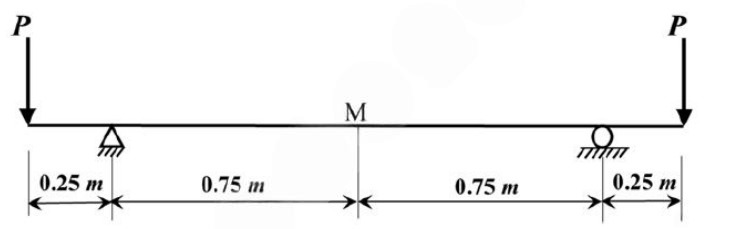
\includegraphics[width=0.5\columnwidth]{fig4.png}
    \caption{}
    \label{fig:placeholder}
\end{figure}

\hfill (GATE PI 2017)

\item A solid circular shaft is subjected to a bending moment $M$ and torque $T$ simultaneously. Neglecting stress concentration effects,  
the equivalent bending moment is expressed as:
\begin{enumerate}
\begin{multicols}{2}
\setlength{\itemsep}{0.3cm}
\item $\frac{M + \sqrt{M^{2} + 4T^{2}}}{2}$
\item $\frac{M}{2} + \sqrt{M^{2} + T^{2}}$
\item $\frac{M + \sqrt{M^{2} + 4T^{2}}}{2}$
\item $\frac{M}{2} + \sqrt{M^{2} + 4T^{2}}$
\end{multicols}
\end{enumerate}
\hfill (GATE PI 2017)

\item A pair of spur gears with $20^\circ$ full\--depth involute teeth is used to transmit $3.5 \ \text{kW}$ of power.  
The pinion rotates at $700 \ \text{rpm}$ and has a pitch circle diameter of $100 \ \text{mm}$.  
Assuming a single pair of teeth in contact, the total force acting on a gear tooth (in kN) is:
\begin{enumerate}
\begin{multicols}{4}
\item 0.347
\item 0.954
\item 1.016
\item 1.302
\end{multicols}
\end{enumerate}
\hfill (GATE PI 2017)

\item A manometer is used for the pressure measurement in a closed tank. The three fluids $f_1$, $f_2$, and $f_3$  
have specific weights $\gamma$, $2\gamma$, and $0.5\gamma$, respectively.  
In order to ensure zero gauge pressure in the tank at the mid\--height level $\brak{h/2}$, the height of the tank $h$ (in m) is \dots

\begin{figure}[H]
    \centering
    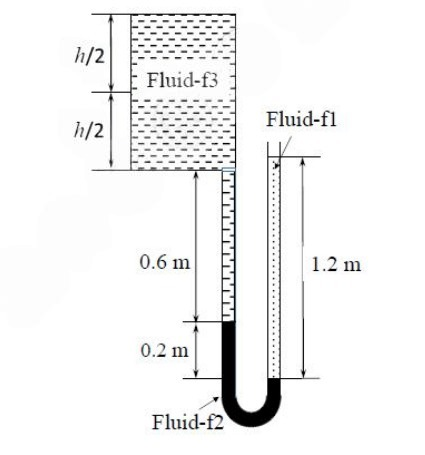
\includegraphics[width=0.4\columnwidth]{fig5.png}
    \caption{}
    \label{fig:placeholder}
\end{figure}

\hfill (GATE PI 2017)

\item A pipeline with variable cross\--section contains water with specific weight $10^4 N/m^3$.  
The flow conditions at two points 1 and 2 along the axis of the pipe are:  
$P_1 = 3\ bar$, $P_2 = 1\ bar$, $V_1$ = 10 m/s, $V_2$ =20 m/s .  
Neglecting frictional losses, for no\--flow condition between the points (as shown), if the height $z_1$ from datum is 1 m,  
then the height $z_2$ (in m) is \dots

\begin{figure}[H]
    \centering
    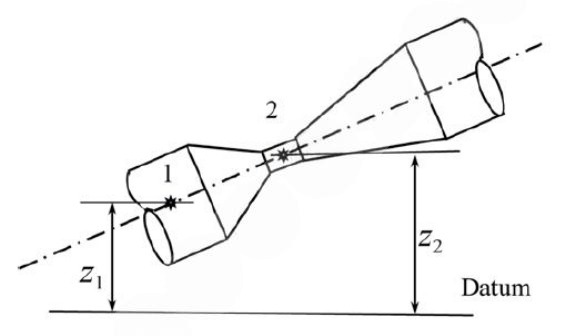
\includegraphics[width=0.4\columnwidth]{fig7.png}
    \caption{}
    \label{fig:placeholder}
\end{figure}


\hfill (GATE PI 2017)

\item A reversible heat engine $E$ operates in a cycle between three reservoirs at  
$T_{1}$ = 500K, $T_{2}$ = 400K and $T_{3} $= 300K.  
The engine receives 10 kJ of heat from reservoir 1 and rejects 3 kJ to reservoir 3.  
The net work output, $W_{{net}}$ (in kJ) from the engine is \dots 

\begin{figure}[H]
    \centering
    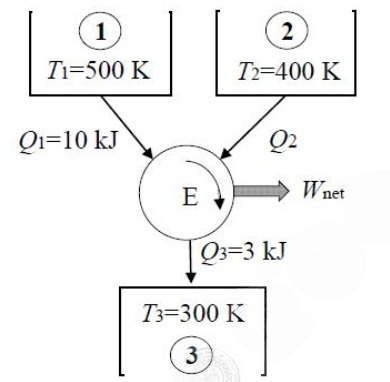
\includegraphics[width=0.5\columnwidth]{fig8.png}
    \caption{}
    \label{fig:placeholder}
\end{figure}

\hfill (GATE PI 2017)

\item A schematic diagram of peripheral milling is shown in figure .
\begin{figure}[H]
    \centering
    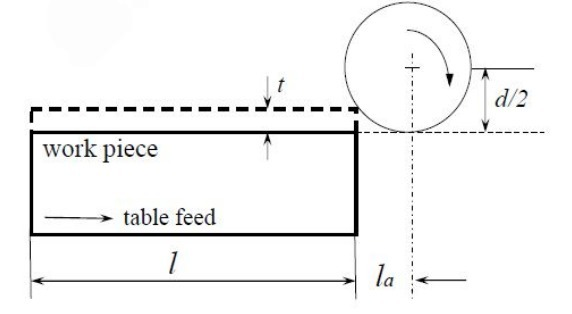
\includegraphics[width=0.4\columnwidth]{fig6.png}
    \caption{}
    \label{fig:placeholder}
\end{figure}


If $t$ is the depth of cut and $d$ is the cutter diameter, the length of approach $l_a$ is:
\begin{enumerate}
\begin{multicols}{2}
\item $\sqrt{d(t - d)}$
\item $d(d - t)$
\item $t(d - t)$
\item $t(t - d)$
\end{multicols}
\end{enumerate}
\hfill (GATE PI 2017)

\item An electrical appliances showroom sells $2400$ ceiling fans in one year ($52$ weeks).  
The holding cost is $10\%$ of the cost of the fan, unit cost = Rs. 600, ordering cost = Rs. 201/order, lead time = 5 weeks.  
The EOQ and reorder level respectively (rounded to next higher integer) are:
\begin{enumerate}
\begin{multicols}{4}
\item 231, 127
\item 38, 231
\item 127, 231
\item 127, 13
\end{multicols}
\end{enumerate}
\hfill (GATE PI 2017)

\item In a calendar year, the demand forecast of motorbikes for June is $200$.  
The actual demand for June and July are $300$ and $350$, respectively.  
Using single exponential smoothing with smoothing constant $0.7$, the forecast for August is \dots

\hfill (GATE PI 2017)

\item In a project, tasks A, B, C, D, E, F, G, H, I, J have given precedence and durations.  
The time required (in days) to complete the project along the critical path is\dots \\

\begin{tabular}[12pt]{ |c| c| } 
    \hline
    {Group I: Aircraft mode} & {Group II: Property}\\ 
    \hline
    P: Short period mode & 1: Coupled roll-yaw oscillations\\
    \hline 
    Q: Wing rock & 2: Angle of attack remains constant \\
    \hline
    R: Phugoid mode & 3: Roll oscillations \\
    \hline   
    S: Dutch roll & 4: Speed remains constant\\
    \hline
\end{tabular}

 
\hfill (GATE PI 2017)

\item The potential production alternatives for manufacturing a product and their unit cost/capacity are given in the table 
Inventory at July end = $100$ units, August demand = $620$ units.  
The minimum total cost (in Rs.) to meet the demand is \dots\\

\begin{table}[htbp]
  \centering
  \caption{Table-3}
  \label{table3}
  \begin{tabular}{cc}

\textbf{Column I} & \textbf{Column II}\\
     (P) Solid state sintering & (1) Carbon nanotube products\\
     (Q) Liquid phase sintering & (2) Mixture of Cu and Zn powder\\
     (R) Spark plasma sintering & (3) iron powder products\\
     (S) Laser sintering & (4) 3D printed products

  \end{tabular}
\end{table}

\hfill (GATE PI 2017)

\item The preparatory and miscellaneous codes used in CNC part programming and the functions are given in the Table. \\

\begin{center}
\begin{tabular}[12pt]{|l|l|}
\hline 
  P.Processes   & 1.Characteristics / Applications \\ \hline
  Q.Gas Metal Arc Welding    & 2.Joining of thick plates \\ \hline
  R.Tungsten Inert Gas Welding &  3.Consumable electrode wire  \\ \hline
  S.Electroslag Welding & 4.Joining of cylindrical dissimilar materials \\ \hline
\end{tabular}
\end{center}

\hfill (GATE PI 2017)

\item A surface $30 mm \times 30 mm$ of an iron block is machined using electrochemical machining.  
For iron: atomic weight $=55.85$, valency $= 2$, density $= 7.860 kg/m^3$.  
If input current is 1000 A and Faraday's constant 96540 C,  
then the feed rate (in mm/min) is \dots (up to two decimal places)   

\hfill (GATE PI 2017)

\item Quality control department of a company maintains a \textit{c}-chart to assess the quality of laptops.  
In this process, twenty laptops are examined randomly. The number of nonconformities observed per laptop is: 

\begin{table}[htbp]
  \centering
  \caption{Table-6}
  \label{table6}
  \begin{tabular}{cc}
\textbf{Products} & \textbf{Polymer}\\

P. Electrical cables & 1. Polyurethane \\
Q. Electrical switches & 2. Poly(methyl methacrylate) \\
R. Optical lenses & 3. Cross-linked polyethylene \\
S. Shoe soles & 4. Phenol formaldehyde resin \\
  
  
  
  \end{tabular}
\end{table}

Based on the data, the upper control limit for the \textit{c}-chart is:  
\dots (up to two decimal places) 

\hfill (GATE PI 2017)

\item The Merchant circle diagram in orthogonal cutting shows various forces associated with a cutting process using a wedge\--shaped tool.  

\begin{figure}[H]
    \centering
    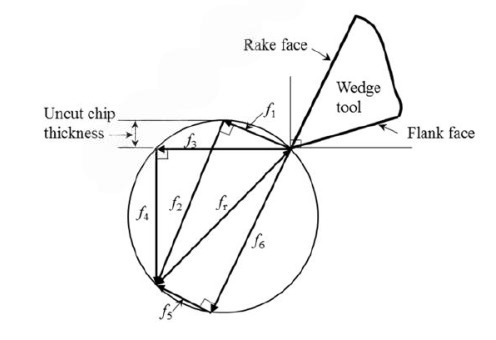
\includegraphics[width=0.5\columnwidth]{fig10.png}
    \caption{}
    \label{fig:placeholder}
\end{figure}

The coefficient of friction can be estimated from the ratio:

\begin{enumerate}
\begin{multicols}{2}
\item $\frac{f_1}{f_2}$
\item $\frac{f_3}{f_4}$
\item $\frac{f_5}{f_6}$
\item $\frac{f_6}{f_5}$
\end{multicols}
\end{enumerate}
\hfill (GATE PI 2017)

\item An air conditioning unit is expected to run continuously. The mean time between failures (MTBF) for this unit is $2000$ h and the mean time to repair (MTTR) is $48$ h.  
The availability of the unit is:  
\dots(up to three decimal places)  

\hfill (GATE PI 2017)

\item A firm manufactures capacitors. The desired specification for the capacitance is $40 \pm 10$ picofarads (pF).  
The process mean is $41$ pF and the estimated standard deviation is $3$ pF (process in control).  
The process capability index $C_{pk}$ is:  
\dots

\hfill (GATE PI 2017)

\item A metallic strip $12$ mm thick is to be rolled using two steel rolls each of $800$ mm diameter.  
No change in width of strip occurs during rolling.  
To achieve $10\%$ reduction in cross\--sectional area, the angle subtended (in degrees) by the deformation zone at the roll center is:
\begin{enumerate}
\begin{multicols}{4}
\item 1.84
\item 3.14
\item 6.84
\item 8.23
\end{multicols}
\end{enumerate}

\hfill (GATE PI 2017)

\item An electron beam welding process uses a $15$ mA beam current at an accelerating voltage of $150$ kV.  
The energy released per second by the beam (in J) is:  
\dots (up to one decimal place) ( 1 Ampere = 6.28 x 10$^{18}$ electrons per second, 1eV = 1.6 x 10$-19$J)  

\hfill (GATE PI 2017)

\item In a machine shop, four jobs need to be assigned to four different machines. The processing time (in hours) is:

\begin{center}
\begin{tabular}{|c|c|c|c|c|c|c|c|c|c|c|c|}
\hline
$x$ & 0 & 1 & 2 & 3 & 4 & 5 & 6 & 7 & 8 & 9 & 10 \\
\hline
$y\brak{x}$ & 5 & 3 & 0 & -5 & -10 & -6 & 0 & 5 & 11 & 18 & 30 \\
\hline
\end{tabular}
\end{center}


The optimal assignment to minimize total time is:
\begin{enumerate}
\item J1$\implies$ M4,\ J2$\implies$ M2,\ J3$\implies$ M3,\ J4$\implies$M1
\item J1$\implies$M2,\ J2$\implies$M1,\ J3$\implies$M4,\ J4$\implies$M3
\item J1$\implies$M2,\ J2$\implies$M1,\ J3$\implies$M3,\ J4$\implies$M4
\item J1$\implies$M4,\ J2$\implies$M2,\ J3$\implies$M1,\ J4$\implies$M3
\end{enumerate}
\hfill (GATE PI 2017)

\item A hose coupling manufacturer has annual production capacity = $2500$ units.  
Selling price/unit = Rs.\ 150, fixed cost = Rs.\ 80{,}000, variable cost/unit = Rs.\ 70.  
If desired annual profit = Rs.\ 20{,}000, the minimum annual quantity to produce is:  
\dots 

\hfill (GATE PI 2017)

\item Schematic diagram of pouring basin and sprue of a gating system is shown in the figure.  
Depth of molten metal in the pouring basin is 100 mm and the height of the sprue is $1500$mm.  



\begin{figure}[H]
    \centering
    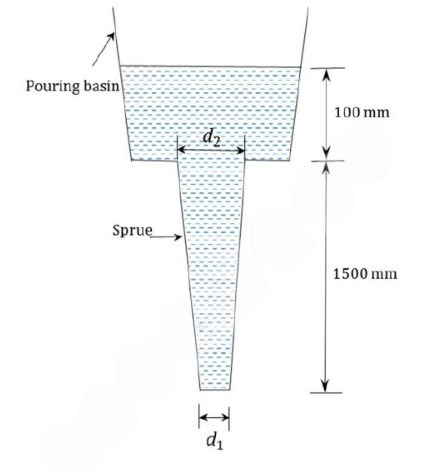
\includegraphics[width=0.3\columnwidth]{fig9.png}
    \caption{}
    \label{fig:placeholder}
\end{figure}

Considering the cross \-- section of the sprue is circular, the ratio $d_{1} : d_{2}$ to avoid aspiration is:

\begin{enumerate}
\begin{multicols}{4}
\item 3:2
\item 5:6
\item 15:16
\item 1:2
\end{multicols}
\end{enumerate}
\hfill (GATE PI 2017)

\item In a numerical control (NC) machine positioning system, the measures of precision are expressed by considering a single axis as shown in the figure.  
If $\sigma$ is standard deviation of the error distribution, then  $l$, $m$ and $n$ are:

\begin{figure}[H]
    \centering
    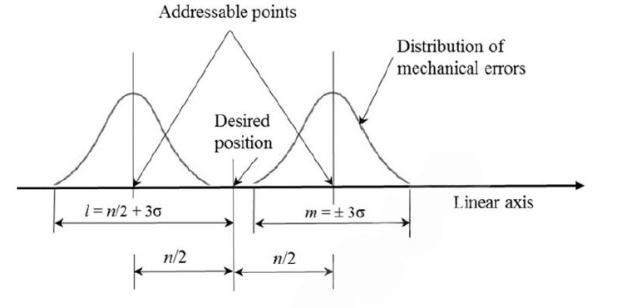
\includegraphics[width=0.5\columnwidth]{fig11.png}
    \caption{}
    \label{fig:placeholder}
\end{figure}

\begin{enumerate}
\item $l=$ Accuracy,\ $m=$ Repeatability,\ $n=$ Control resolution
\item $l=$ Repeatability,\ $m=$ Accuracy,\ $n=$ Control resolution
\item $l=$ Control resolution,\ $m=$ Repeatability,\ $n=$ Accuracy
\item $l=$ Accuracy,\ $m=$ Control resolution,\ $n=$ Repeatability
\end{enumerate}
\hfill (GATE PI 2017)

\item In a machining operation with turning tool, the tool life ($T$) is related to cutting speed $v$ (m/s), feed $f$ (mm) and depth of cut $d$ (mm) as:  
\begin{align*}
T = C\, v^{-0.25} f^{-0.9} d^{-0.15}
\end{align*}
where $C$ is a constant. The suggested values are $v = 1.5 \ \text{m/s}$, $f = 0.25 \ \text{mm}$ and $d = 3 \ \text{mm}$ for normal rough turning.  
If the operation is performed at twice the cutting speed and other parameters remain unchanged,  
the corresponding percentage change in tool life is:  
\dots

\hfill (GATE PI 2017)

\item The annual demand of wrist watches produced on an assembly line is $103{,}125$ units.  
The line operates $50$ weeks/year, $5$ shifts/week, and $7.5$ hours/shift.  
The uptime efficiency of the line is $99\%$.  
The cycle time ($T_c$) of the assembly line (in minutes/unit) is:  
\dots (up to two decimal places)  

\hfill (GATE PI 2017)

\item In a gear manufacturing company, three orders P, Q and R are to be processed on a hobbing machine.  
The orders were received in the sequence P\--Q\--R. The table indicates the process time remaining and due date for each order: \\

\begin{center}
\begin{tabular}{lcc}
 & {Automat} & {Center Lathe} \\
\hline
Machine Setup Time (min) & 120 & 30 \\ \hline
Machine Setup Cost (Rs./min) & 800 & 150 \\ \hline
Machining Time per piece (min) & 2 & 25 \\ \hline
Machining Cost (Rs./min) & 500 & 100 \\ \hline \\
\end{tabular}
\end{center}


Considering today as Day 10 of the production calendar,  
the sequence scheduled using the 'Critical Ratio' rule is:
\begin{enumerate}
\begin{multicols}{2}
\item P\--Q\--R
\item P\--R\--Q
\item Q\--P\--R
\item Q\--R\--P
\end{multicols}
\end{enumerate}
\hfill (GATE PI 2017)

\item She has a sharp tongue and it can occasionally turn
\begin{enumerate}
\begin{multicols}{4}
\item hurtful
\item left
\item methodical
\item vital
\end{multicols}
\end{enumerate}
\hfill (GATE PI 2017)

\item I \dots made arrangements had I \dots informed earlier.
\begin{enumerate}
\begin{multicols}{2}
\item could have, been
\item would have, being
\item had, have
\item had been, been
\end{multicols}
\end{enumerate}
\hfill (GATE PI 2017)

\item In the summer, water consumption is known to decrease overall by $25\%$.  
A Water Board official states that in the summer household consumption decreases by $20\%$, while other consumption increases by $70\%$.  

Which of the following statements is correct?
\begin{enumerate}
\item The ratio of household to other consumption is $8/17$
\item The ratio of household to other consumption is $1/17$
\item The ratio of household to other consumption is $17/8$
\item There are errors in the official's statement
\end{enumerate}
\hfill (GATE PI 2017)

\item $40\%$ of deaths on city roads may be attributed to drunken driving.  
The number of degrees needed to represent this as a slice of a pie chart is:
\begin{enumerate}
\begin{multicols}{4}
\item 120
\item 144
\item 160
\item 212
\end{multicols}
\end{enumerate}
\hfill (GATE PI 2017)

\item Some tables are shelves.  
Some shelves are chairs.  
All chairs are benches.  

Which of the following conclusions can be deduced from the preceding sentences?  
i. At least one bench is a table.  \\
ii. At least one shelf is a bench.  \\
iii. At least one chair is a table.  \\
iv. All benches are chairs.\\
\begin{enumerate}
\begin{multicols}{4}
\item Only i
\item Only ii
\item Only ii and iii
\item Only iv
\end{multicols}
\end{enumerate}
\hfill (GATE PI 2017)

\item "If you are looking for a history of India, or for an account of the rise and fall of the British Raj,  
or for the reason of the cleaving of the subcontinent into two mutually antagonistic parts and the effects this mutilation will have in  
the respective sections, and ultimately on Asia, you will not find it in these pages; for though I have spent a lifetime in the country,  
I lived too near the seat of events, and was too intimately associated with the actors, to get the perspective needed for the  
impartial recording of these matters." 

Here, the word 'antagonistic' is closest in meaning to:
\begin{enumerate}
\begin{multicols}{4}
\item impartial
\item argumentative
\item separated
\item hostile
\end{multicols}
\end{enumerate}
\hfill (GATE PI 2017)

\item S,T,U,V,W,X,Y and Z are seated around a circular table.  
T's neighbours are Y and V. Z is seated third to the left of T and second to the right of S. U's neighbours are S and Y;  
and T and W are not seated opposite each other.  

Who is third to the left of V?
\begin{enumerate}
\begin{multicols}{4}
\item X
\item W
\item U
\item T
\end{multicols}
\end{enumerate}
\hfill (GATE PI 2017)

\item Trucks (10 m long) and cars (5 m long) go on a single lane bridge.  
There must be a gap of at least 20 m after each truck and a gap of at least 15 m after each car.  
Trucks and cars travel at a speed of 36 km/hr.  

If cars and trucks go alternately, the maximum number of vehicles that can use the bridge in one hour is:
\begin{enumerate}
\begin{multicols}{4}
\item 1440
\item 1200
\item 720
\item 600
\end{multicols}
\end{enumerate}
\hfill (GATE PI 2017)

\item There are 3 Indians and 3 Chinese in a group of 6 people.  
How many subgroups of this group can be chosen so that every subgroup has at least one Indian?
\begin{enumerate}
\begin{multicols}{4}
\item 56
\item 52
\item 48
\item 44
\end{multicols}
\end{enumerate}
\hfill (GATE PI 2017)

\item A contour line joins locations having the same height above mean sea level.  
The following is a contour plot of a geographical region. Contour lines are shown at 25 m intervals.  

\begin{figure}[H]
    \centering
    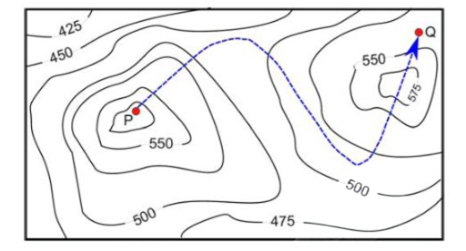
\includegraphics[width=0.5\columnwidth]{fig12.png}
    \caption{}
    \label{fig:placeholder}
\end{figure}

The path from $P$ to $Q$ is best described by:
\begin{enumerate}
\begin{multicols}{2}
\item Up\--Down\--Up\--Down
\item Down\--Up\--Down\--Up
\item Down\--Up\--Down
\item Up\--Down\--Up
\end{multicols}
\end{enumerate}
\hfill (GATE PI 2017)

\end{enumerate}

\end{document}